\documentclass[11pt]{article}
\usepackage{graphicx} %for displaying images
\usepackage{float}
\usepackage{listings}
\usepackage{color}


\definecolor{dkgreen}{rgb}{0,0.6,0}
\definecolor{gray}{rgb}{0.5,0.5,0.5}
\definecolor{mauve}{rgb}{0.58,0,0.82}

\lstset{frame=tb,
	language=Python,
	aboveskip=3mm,
	belowskip=3mm,
	showstringspaces=false,
	columns=flexible,
	basicstyle={\small\ttfamily},
	numbers=none,
	numberstyle=\tiny\color{gray},
	keywordstyle=\color{blue},
	commentstyle=\color{dkgreen},
	stringstyle=\color{mauve},
	breaklines=true,
	breakatwhitespace=true,
	tabsize=3
}

%----------------------------------------------------------------------------------------
%	TITLE SECTION
%----------------------------------------------------------------------------------------
\title{	
	\normalfont\normalsize
	\textsc{Old Dominion University}\\ % Your university, school and/or department name(s)
	\vspace{25pt} % Whitespace
	\rule{\linewidth}{0.5pt}\\ % Thin top horizontal rule
	\vspace{20pt} % Whitespace
	{\huge Assignment Three}\\ % The assignment title
	\vspace{12pt} % Whitespace
	\rule{\linewidth}{2pt}\\ % Thick bottom horizontal rule
	\vspace{20pt} % Whitespace
}
\author{\LARGE Joshua Gahan} % Your name
\date{\normalsize\today} % Today's date (\today) or a custom date

\begin{document}
	\pagenumbering{gobble}
	\maketitle %render title
	\newpage
	\pagenumbering{arabic}
	
	\section{HTML Collection}
	\hspace{10mm} We collected the HTML and text representations of the URLS we collected in the prior assignment. Two files were created per good url-- a HTML representation and a text representation of each file. 
	\subsection{Retrieval of HTML/text}
	\begin{lstlisting}
	for url in data:
	    count += 1
	    try:
	        html = requests.get(url, timeout=15)
	        md5 = hash(str(url).strip()) + sys.maxsize  # we has sys.maxsize here so we don't produce negative nums as hash
        	with open("./rawhtml/%s.html" % md5, 'w') as outFile:
	            outFile.write(html.text)
	
	        extractor = Extractor(html=html.text)
	        with open("./texthtml/%s.txt" % md5, 'w') as outFile:
	           outFile.write(extractor.getText())
	
	        data[url]['%s' % "html_raw_filename"] = "%s.html" % md5
	        data[url]['%s' % "html_text_filename"] = "%s.txt" % md5
	    except Exception as e:
	        print("Error:", str(e), ":  %s" % url)
	        with open('a3_html_get_ErrorURLs.txt', 'a') as err:
	           err.write("%s\n" % url)
	    if count % 50 == 0:
	       print("%d Links have been processed" % count)
	\end{lstlisting}
	\hspace{10mm} We use the requests library to fetch the HTML representation of the page. We calculate the hash of the URI for use later as a unique file name. Utilizing the boilerplate library we then strip the the text from the HTML with the Extractor. Finally we store the file entries in our urlsClean.json index (created in a prior assignment). 
	\begin{figure}[h!]
		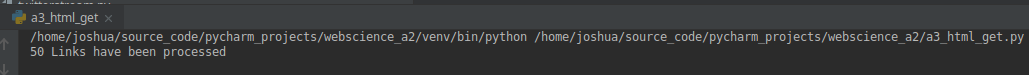
\includegraphics[scale=0.5]{resources/a3_html_get_run.png}
		\caption{HTML/Text Console output}
	\end{figure}
	\section{Query Term and TF-IDF}
	\hspace{10mm} We searched our corpus for documents that contained the word "Mueller" and calculated TF-IDF for those documents. Searching of the documents was accomplished by piping a Linux grep call to a text file (grep.txt) and then adding appropriate entries to urlsClean.json (functionality not shown, but found within grep\_copy.py). We then calculate the TF-IDF scores our URIs. An important point of note here is TF-IDF was computed from our own collected corpus of 4500 URIs and not from the estimates provided by a search engine. 
	\subsection{Calculation of TF-IDF}
	\begin{lstlisting}
	wordcount = ""
	goodURL = json.load(open("urlsClean.json"))
	docs_in_corpus = 0
	docs_where_term_appears = 0
	
	for url in goodURL:
	    docs_in_corpus += 1
	
	for url in goodURL:
	    try:
	       x = goodURL[url]["keywords"]["Mueller"]
	       docs_where_term_appears += 1
	    except Exception as e:
	       pass
	
	for url in goodURL:
	    try:
	        x = goodURL[url]["keywords"]
	        with open("./texthtml/" + goodURL[url]["html_text_filename"]) as file:
	           finalCheck = file.read()
	           wordcount = Counter(finalCheck.split())
	
	           count = 0
	           for key in wordcount:
	              count += wordcount[key]
	
	           tf = finalCheck.count("Mueller") / count #tf = term frequency
	           goodURL[url]["keywords"]["Mueller"]["TF"] = tf
	           idf = math.log(docs_in_corpus/(1 + docs_where_term_appears), 2) # 1+ on inverse doc frequency to prevent x/0 errors
	           goodURL[url]["keywords"]["Mueller"]["IDF"] = idf
	           goodURL[url]["keywords"]["Mueller"]["TF-IDF"] = tf * idf
	\end{lstlisting}
	\hspace{10mm} We began by counting the number of documents we have and the number of documents where "Mueller" appears. The x = goodURL[url].. will throw an exception if that key isn't there, and we take advantage of this here and below. Within the primary loop, we open the file and estimate the word count of the file. This is accomplished by dumping the the file into a Counter (a superset of the dictionary class) and looping through for a count. We then calculate the TF by dividing the integer returned by finalCheck.count (This returns the number of occurrences of a string) by the number of words in the document (the count variable) We take our found Term Frequency and divide it by one plus the number of documents where the term occurs, taking the $log_2$ of the result to get our IDF. Finally we get our TF-IDF by simply multiplying the TF by the IDF. Below we show what our JSON representation looks like after applying this step and the one above. 
	\begin{figure}[h!]
		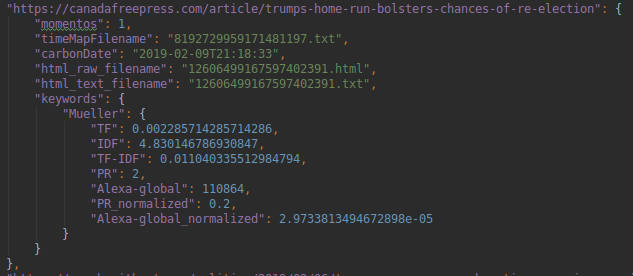
\includegraphics[scale=0.5]{resources/tf-idf-json.png}
		\caption{Example of our data after the above operations. Note that PR/Alexa calculations are completed below}
	\end{figure}
	\section{Page Rank and Alexa}
	\hspace{10mm} We selected twenty-two of our URIs that were found to contain our search term and using http://www.prchecker.info/check\_page\_rank.php and the Alexa website we manually calculated the Page Rank and Alexa rank for each of them. These were stored in urlsClean.json along with the rest of the data. These scores were then normalized and the normalized scores were also stored in urlsClean.json
	\subsection{PR/Alexa score normalization}
	\begin{lstlisting}
	def featurescaling(x, x_min, x_max):
	    return ((x - x_min)/ (x_max - x_min))
	    
	goodURL[url]["keywords"]["Mueller"]["PR_normalized"] = featurescaling(goodURL[url]["keywords"]["Mueller"]["PR"],0,10) #normalizing data
	x = 1 / featurescaling(goodURL[url]["keywords"]["Mueller"]["Alexa-global"],1,10000000) #alex scores are in reverse we are adjusting for this.
	goodURL[url]["keywords"]["Mueller"]["Alexa-global_normalized"] = featurescaling(x, 1, 3000000) #numbers are abitrary to force our Alexa ranks to < 1
	\end{lstlisting}
	\hspace{10mm} Of note here is the normalization of Alexa scores. Alexa page rank scores are ranked such that a Alexa page rank of one would represent the world's most popular site, where rank of one hundred would be the hundredth most popular. For this reason we divide one by the normalized Alexa score and renormalize the resulting value. Note that the large x\_max values are arbitrary values to force the Alex page rank to normalize between zero and one. 
	  
	\section{Kendall $\tau$-b and Pearson correlation scores}
	\hspace{10mm} We then calculated the correlation between each pair of the three found ranks (TF-IDF,Page Rank, Alexa) utilizing the Kendall $\tau$-b and Pearson correlation methods. 
	\subsection{Kendall $\tau$-b and Pearson calculations }
	\begin{lstlisting}
	def getTaub_or_Pearson(tfidf_PR_Alexa_list, desiredIndextoSortBy, IndextoCompareAgainst, getPearsonCorrelation = False):
	    pairs = []
	    sort_list = []
	    compar_list = []
	    ''' Note: some logic omitted here for selecting which list to sort by and compare against. '''
	    if getPearsonCorrelation == False:
	        result = stats.kendalltau(sort_list, compar_list)
	    else:
	        result = stats.pearsonr(sort_list,compar_list)
	    return result
	    
	#tau calculations
	#generate a 2d list containing the normalized TFIDF, PR, and Alexa ranks for selected URLs
	pairs = []
	for url in goodURL:
	   try:
	        pairs.append([goodURL[url]["keywords"]["Mueller"]["TF-IDF"],goodURL[url]["keywords"]["Mueller"]["PR_normalized"], goodURL[url]["keywords"]["Mueller"]["Alexa-global_normalized"]])
    	except Exception as e:
	        pass
	
	#calculate our tau-b and p scores
	tfidf_PR_taub_and_pvalue = getTaub_or_Pearson(pairs, 0, 1)
	tfidf_Alexa_taub_and_pvalue = getTaub_or_Pearson(pairs, 0, 2)
	PR_Alexa_taub_and_pvalue = getTaub_or_Pearson(pairs, 1, 2)
	
    #calculate Pearson scores	
	tfidf_PR_pearson_and_pvalue = getTaub_or_Pearson(pairs, 0, 1, True)
	tfidf_Alexa_pearson_and_pvalue = getTaub_or_Pearson(pairs, 0, 2, True)
	PR_Alexa_pearson_and_pvalue = getTaub_or_Pearson(pairs, 1, 2, True)
	\end{lstlisting}
	\hspace{10mm} For calculating these correlations we used the stat module of the Scipy library.  We construct a 2D array (pairs) of the form [[TF-IDF],[PageRank],[Alexa]] containing the respective scores for each url such that for ${i_0j_0, i_0j_1 , i_0j_2}$ refer to the TF-IDF, PageRank, and Alexa scores of the first URL respectively. 
	
	\section{Findings}
	\hspace{10mm} Below is the data that we have found (rounded to 7 significant figures) for TFIDF and Page Rank calculation. Strictly from looking at our two tables, it does not appear that there is a very strong correlation between the estimated Page rank and the TFIDF. Page Rank consistently puts large media outlets such as Yahoo, BBC, and the Atlantic on top, and yet for TFIDF our most relevant results were small to medium sized news and opinion outlets. In particular https//palmerreport.com is near the bottom of the Page Rank list, but the very top entry in TFIDF. There is a some agreement between them however, with both TFIDF and PR agreeing that blog "lifeofanelpasowoman.com" is of low importance. 
	\subsection{TFIDF and Page Rank Tabular Data }
	\newpage
	\begin{table}[h!]
		\begin{tabular}{llll}
			TFIDF     & TF        & IDF       & URL                                                                                                                                   \\
			0.0921784 & 0.019084  & 4.8301468 & https://www.palmerreport.com/analysis/jr-bad-habit-donald-trump-catch/15870/                                                          \\
			0.0911348 & 0.0188679 & 4.8301468 & https://www.newsmax.com/                                                                                                              \\
			0.0761198 & 0.0157593 & 4.8301468 & https://www.cnbc.com/2018/11/07/trump-says-attorney-general-jeff-sessions-resigns.html                                                \\
			0.0540688 & 0.011194  & 4.8301468 & https://www.yahoo.com/news/matt-whitaker-headed-trump-hotel-083018883.html?.tsrc=fauxdal                                              \\
			0.0456248 & 0.0094458 & 4.8301468 & http://www.msn.com/en-us/news/politics/trump-advisers-lied-over-and-over-again-mueller-says-the-question-is-why/ar-BBSN7ef?ocid=st    \\
			0.0146962 & 0.0030426 & 4.8301468 & https://www.nbcnews.com/think/opinion/trump-s-state-union-had-same-mistake-nixon-s-ending-ncna968421                                  \\
			0.0135678 & 0.002809  & 4.8301468 & https://countzpr.com/2019/02/09/don-lemon-tears-into-president-for-past-harassment-of-barack-obama/                                   \\
			0.0133799 & 0.0027701 & 4.8301468 & https://tacticalinvestor.com/clinton-claims-she-didnt-know-about-the-dossier                                                          \\
			0.0119706 & 0.0024783 & 4.8301468 & https://www.usatoday.com/story/opinion/2019/01/22/donald-trump-pursued-business-deal-russia-hid-voters-editorials-debates/2642773002/ \\
			0.0112068 & 0.0023202 & 4.8301468 & https://www.yahoo.com/news/trump-ordered-justice-department-draft-122132539.html?.tsrc=fauxdal                                        \\
			0.0110403 & 0.0022857 & 4.8301468 & https://canadafreepress.com/article/trumps-home-run-bolsters-chances-of-re-election                                                   \\
			0.0096218 & 0.001992  & 4.8301468 & https://grondamorin.com/2019/02/06/house-committee-is-set-to-go-after-president-trumps-tax-returns/                                   \\
			0.0080675 & 0.0016702 & 4.8301468 & https://www.businessinsider.com/steele-dossier-allegations-trump-russia-mueller-investigation-2019-1                                  \\
			0.0080102 & 0.0016584 & 4.8301468 & https://redrightvideos.com/the-truth-about-the-fbis-counter-intelligence-investigation-into-trump/                                    \\
			0.0078603 & 0.0016273 & 4.8301468 & https://www.nbcnews.com/think/opinion/trump-s-lawyers-yes-including-rudy-giuliani-have-tough-job-ncna964871                           \\
			0.0063177 & 0.001308  & 4.8301468 & https://www.theatlantic.com/magazine/archive/2019/03/impeachment-trump/580468/                                                        \\
			0.006091  & 0.001261  & 4.8301468 & https://www.bbc.co.uk/news/world-us-canada-47061509                                                                                   \\
			0.0055265 & 0.0011442 & 4.8301468 & https://www.sandiegouniontribune.com/news/us-politics/la-na-pol-trump-impeachment-investigations-20190210-story.html                  \\
			0.0051659 & 0.0010695 & 4.8301468 & http://nymag.com/intelligencer/2019/02/trump-tax-cuts-doing-opposite-of-promised-corporate-cash-accountants.html                      \\
			0.0026194 & 0.0005423 & 4.8301468 & https://lifeofanelpasowoman.com/2019/02/10/trump-is-coming-to-el-paso-etc/                                                            \\
			0.0025857 & 0.0005353 & 4.8301468 & https://www.cnbc.com/2019/02/08/firm-owned-by-trumps-longtime-bodyguard-has-received-225000-from-rnc.html                            
		\end{tabular}
	\caption{TFIDF Finding}
	\end{table}
	\newpage
	\begin{table}[h!]
		\begin{tabular}{ll}
			PR & URL                                                                                                                                   \\
			9  & https://www.yahoo.com/news/trump-ordered-justice-department-draft-122132539.html?.tsrc=fauxdal                                        \\
			9  & https://www.yahoo.com/news/matt-whitaker-headed-trump-hotel-083018883.html?.tsrc=fauxdal                                              \\
			9  & https://www.bbc.co.uk/news/world-us-canada-47061509                                                                                   \\
			8  & https://www.theatlantic.com/magazine/archive/2019/03/impeachment-trump/580468/                                                        \\
			8  & https://www.nbcnews.com/think/opinion/trump-s-state-union-had-same-mistake-nixon-s-ending-ncna968421                                  \\
			8  & https://www.nbcnews.com/think/opinion/trump-s-lawyers-yes-including-rudy-giuliani-have-tough-job-ncna964871                           \\
			8  & http://www.msn.com/en-us/news/politics/trump-advisers-lied-over-and-over-again-mueller-says-the-question-is-why/ar-BBSN7ef?ocid=st    \\
			8  & https://www.usatoday.com/story/opinion/2019/01/22/donald-trump-pursued-business-deal-russia-hid-voters-editorials-debates/2642773002/ \\
			7  & https://www.businessinsider.com/steele-dossier-allegations-trump-russia-mueller-investigation-2019-1                                  \\
			7  & https://www.cnbc.com/2019/02/08/firm-owned-by-trumps-longtime-bodyguard-has-received-225000-from-rnc.html                             \\
			7  & https://www.cnbc.com/2018/11/07/trump-says-attorney-general-jeff-sessions-resigns.html                                                \\
			7  & http://nymag.com/intelligencer/2019/02/trump-tax-cuts-doing-opposite-of-promised-corporate-cash-accountants.html                      \\
			6  & https://www.sandiegouniontribune.com/news/us-politics/la-na-pol-trump-impeachment-investigations-20190210-story.html                  \\
			6  & https://www.newsmax.com/                                                                                                              \\
			2  & https://canadafreepress.com/article/trumps-home-run-bolsters-chances-of-re-election                                                   \\
			0  & https://countzpr.com/2019/02/09/don-lemon-tears-into-president-for-past-harassment-of-barack-obama/                                   \\
			0  & https://redrightvideos.com/the-truth-about-the-fbis-counter-intelligence-investigation-into-trump/                                    \\
			0  & https://grondamorin.com/2019/02/06/house-committee-is-set-to-go-after-president-trumps-tax-returns/                                   \\
			0  & https://www.palmerreport.com/analysis/jr-bad-habit-donald-trump-catch/15870/                                                          \\
			0  & https://tacticalinvestor.com/clinton-claims-she-didnt-know-about-the-dossier                                                          \\
			0  & https://lifeofanelpasowoman.com/2019/02/10/trump-is-coming-to-el-paso-etc/                                                           
		\end{tabular}
		\caption{PageRank Finding}
		\label{my-label}
	\end{table}
	\newpage
	\subsection{Kendall $\tau$-b and Pearson correlations}
	\hspace{10mm} We have compared the each of our three metrics against each other using Kendall $\tau$-b and Pearson correlations between each. The following graphs represent our finding. 
	\begin{figure}[H]
		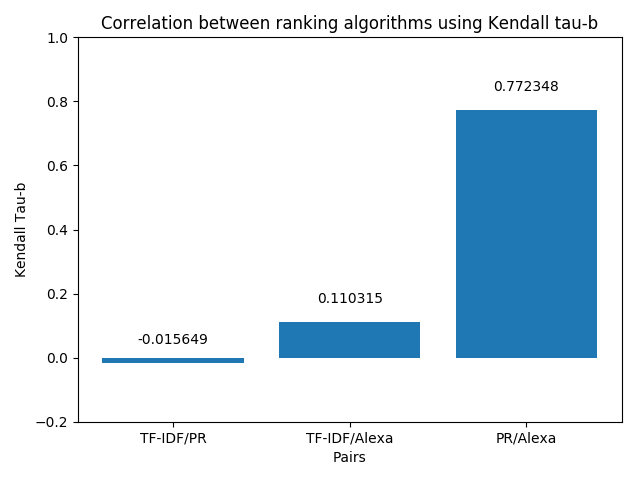
\includegraphics[scale=0.5]{resources/kendall-taub.png}
		\caption{Kendall $\tau$-b}
	\end{figure}
	\begin{figure}[H]
		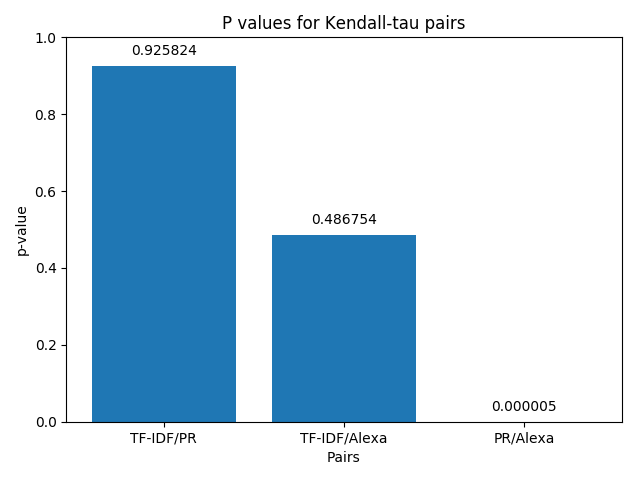
\includegraphics[scale=0.5]{resources/kendall_taub_p.png}
		\caption{Kendall $\tau$-b $p$ scores}
	\end{figure}
	\begin{figure}[H]
		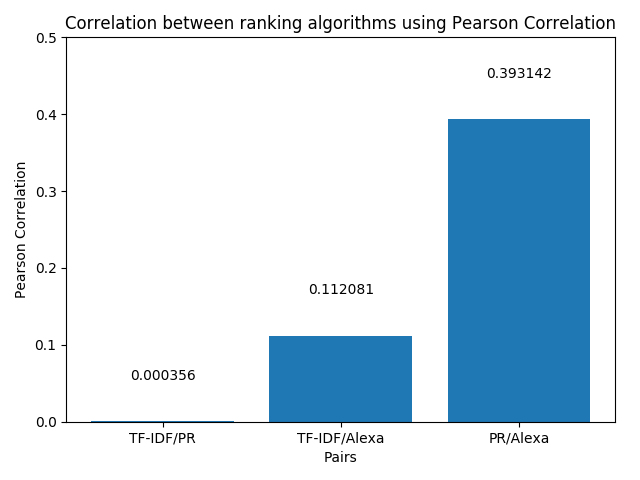
\includegraphics[scale=0.5]{resources/pearson.png}
		\caption{Pearson Correlation}
	\end{figure}
	\begin{figure}[H]
		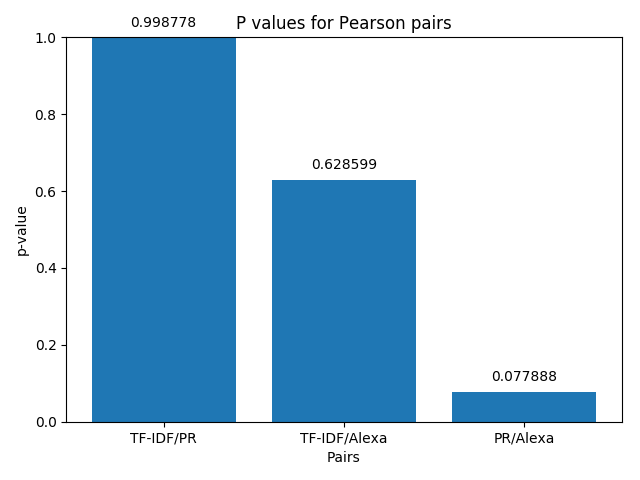
\includegraphics[scale=0.5]{resources/pearson_p.png}
		\caption{Pearson Correlation $p$ values}
	\end{figure}
	\newpage
	\subsection{A Summary of Correlations}
	\subsubsection{TF-IDF/PR}
	\hspace{10mm} From the graphs it is obvious that there is a very weak correlation between TF-IDF and our estimated Page Rank for both Pearson and Kendall correlations. It should be noted that the high $p$ value here also does not rule out the null hypothesis for the comparision of these two metrics. 
	\subsubsection{TF-IDF/Alexa}
	\hspace{10mm} We have obtained similar results by comparing the TFIDF against the Alexa rank.  As above, we have a weak correlation coupled with a high $p$ value for both the Kendall and Pearson correlation scores. 
	\subsubsection{PR/Alexa}
	\hspace{10mm} Our only statistically significant finding was that there is indeed a very strong correlation between our estimated Page Rank and the Alexa rank for both the Kendall $\tau$-b and Pearson correlation scores. In addition we find that the $p$ of the Pearson correlation is marginally significant at $~0.07$. the $p$ of the Kendall $\tau$-b was found to be highly significant ($p=5.0*10^{-6})$) for the correlation between estimated Page Rank and Alexa Rank. 
	\section{Conclusion}
	\hspace{10mm} As stated above we were only able to show statistically significant correlation between Page Rank and Alexa rank. Our high $p$ values for TF-IDF pairings however does not rule out the null-hypothesis. It is entirely possible that our TF-IDF correlations have been skewed by the way we calculated our data. For TF-IDF the data has been calculated against our own corpus of URIs, including for document frequency. This means that the TF-IDF we have generated does not necessarily reflect what might be in the wild. In particular our document frequency was again drawn from within our own corpus. By comparison The Page Rank estimator we used as well as Alexa have scores that are based on (in theory) larger data sets, as well as having their scores be based on the root domain of the URL.  None the less, it is perhaps not a fair comparison to compare TF-IDF to Page Rank or Alexa, as it serves a different purpose. TFIDF is used to identify how important a resource might be to a query, but its speaks nothing of the 'importance' or popularity of a site as Page Rank and Alexa Rank do. A site may indeed rank very high for Alexa or Pagerank, but contain relatively little data relevant to the information you are querying for. Thus, each serves its own role, but not too much can be made of the importance of one over the other, or correlations between them. 

\end{document}